%!TEX program = xelatex
\documentclass[cn,hazy,pku,12pt,normal,math=newtx,cite=super]{elegantnote}
\title{溶解热的测定}

\author{刘松瑞 \quad 2100011819 \\ 组号:24 \quad 组内编号:5}
\institute{化学与分子工程学院}

\expdate{\zhdate{2023/11/23}}
\temperature{16.9 \si{^{\circ}C}}
\pressure{101.76 \si{kPa}}

\usepackage{gensymb}
\usepackage{array}
\usepackage{subfigure}
\usepackage[fontset=windows]{ctex}
\usepackage{graphicx}
\usepackage{float}
\usepackage{caption}
\usepackage{multirow}
%\usepackage{subfig}
%\usepackage{float}
\begin{document}

\maketitle

\keywords{积分溶解热\quad硝酸钾\quad电热补偿法}

\abstracts{
    本实验利用了电热补偿法测定了硝酸钾在不同浓度的水溶液中的溶解热,绘制了 $T-t$ 图、$Q_s-n_0$ 图、$Q_s^{-1}-n_0^{-1}$ 图以及 $Q_s-n_0^{-1}$ 图,并拟合了 $Q_s^{-1}-n_0^{-1}$ 以及 $Q_s-n_0^{-1}$ 的线性关系。通过经验式,
    得到 $Q_S^0 = 47.6\ {\rm kJ/mol} $、$
    n_0  = 0.078\ {\rm mol/kJ}$
    , 并与真实值相比较,并进一步地计算了其他溶解过程的热效应。
}

\newpage


\section{引言}

\subsection{实验目的与原理}

实验目的与原理详见预习报告图~\ref{1}。 \cite{pcl2002}

\begin{figure}[htbp]
    \centering
    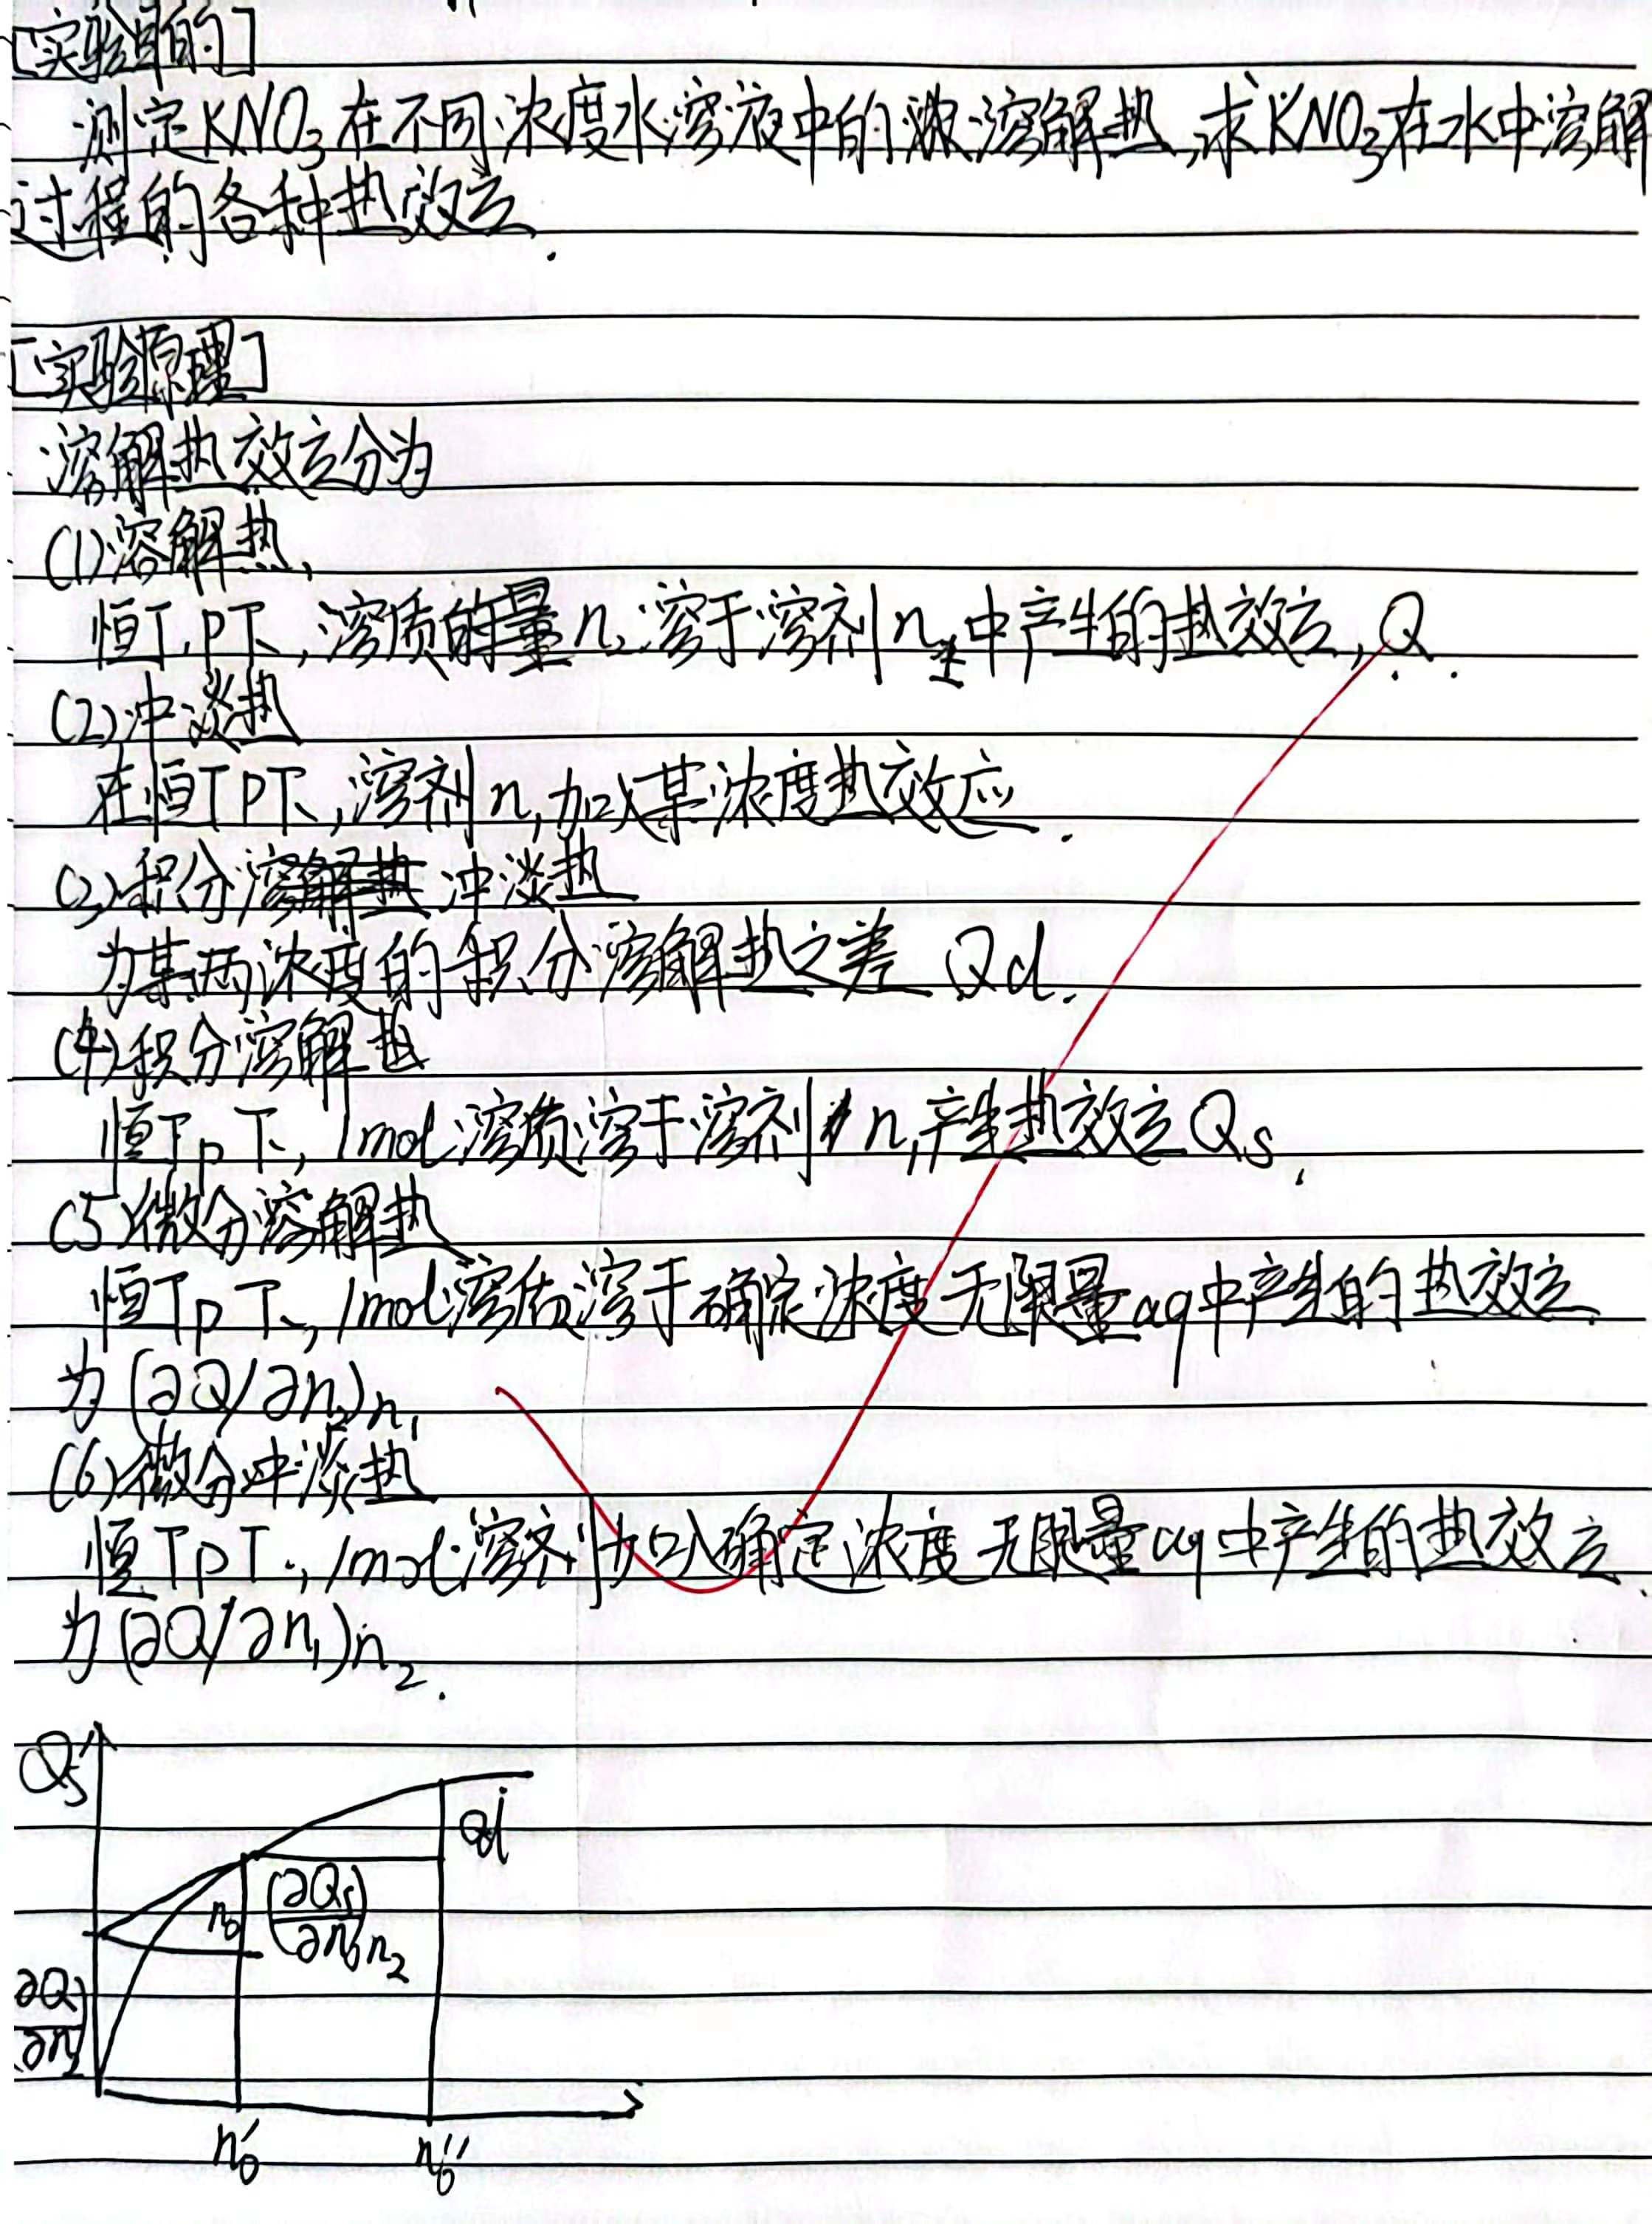
\includegraphics[width = .70\textwidth]{image/yxbg_1.jpg}
    \caption{实验的目的与原理}\label{1}
\end{figure}

\subsection{实验方法}

通过数字温差仪进行两轮实验,计算硝酸钾的溶解热,作图探究 $Q_s$ 与 $n_0$ 关系。

\section{实验部分}

\subsection{实验步骤}
\subsubsection{第一轮实验}

\begin{enumerate}
    \item  用容量瓶准确量取 500.00 mL 去离子水,加入保温瓶中,连接好仪器。
    \item  在分析天平上准确称取 10 g 左右硝酸钾,打开电磁搅拌器,待示数稳定后将温差置零,
    使用软件记录体系温度-时间关系
    \item  打开加料口塞子,通过漏斗加入样品,盖好盖子,待温度
    降至最低点,读数稳定变化后,记录一段平台期,测定溶液电阻。
    \item  打开电阻丝加热开关,记录时间及电流,待温度上升至原温度后断开加热,记录一段平台期。
    \item  用相同方法再加入 3 个样品
\end{enumerate}

\subsubsection{第二轮实验}

\begin{enumerate}
    \item  按照第一轮实验的方法,先在去离子水中加入 10 g 硝酸钾,再依次加入 3 g, 3 g, 4 g, 7 g, 13 g, 30 g 硝酸钾
    \item  作出 $1/Q_s - 1/n_0$ 图。
\end{enumerate}

\subsection{仪器与药品}

\begin{enumerate} %有序列表
    \item 试剂 \\   氯化钾,去离子水。
    \item 仪器 \\   广口保温瓶,磁子,电磁搅拌器,数字温差仪,加热电阻丝,直流稳压电
    源,漏斗,秒表,500 mL 容量瓶,公用万用表。
\end{enumerate}

\section{实验现象与数据处理}
\subsection{溶液浓度计算}
我们使用 $n_0$ 来计算溶液的浓度,由下式可得加入溶质质量与 $n_0$ 的关系。
\begin{equation}\label{001}
    n_0 = \frac{n_1}{n_2} = \frac{0.9988\ g/mL \cdot 500\ mL / 18.016\ g/mol}{m/101.1\ g/mol} = \frac{2802}{m}
\end{equation}
\subsection{第一轮实验}
称取 10 g 左右硝酸钾加入去离子水,重复四组,记录温度-时间关系图如图 \ref{2}。

\begin{figure}[htbp]
    \centering
    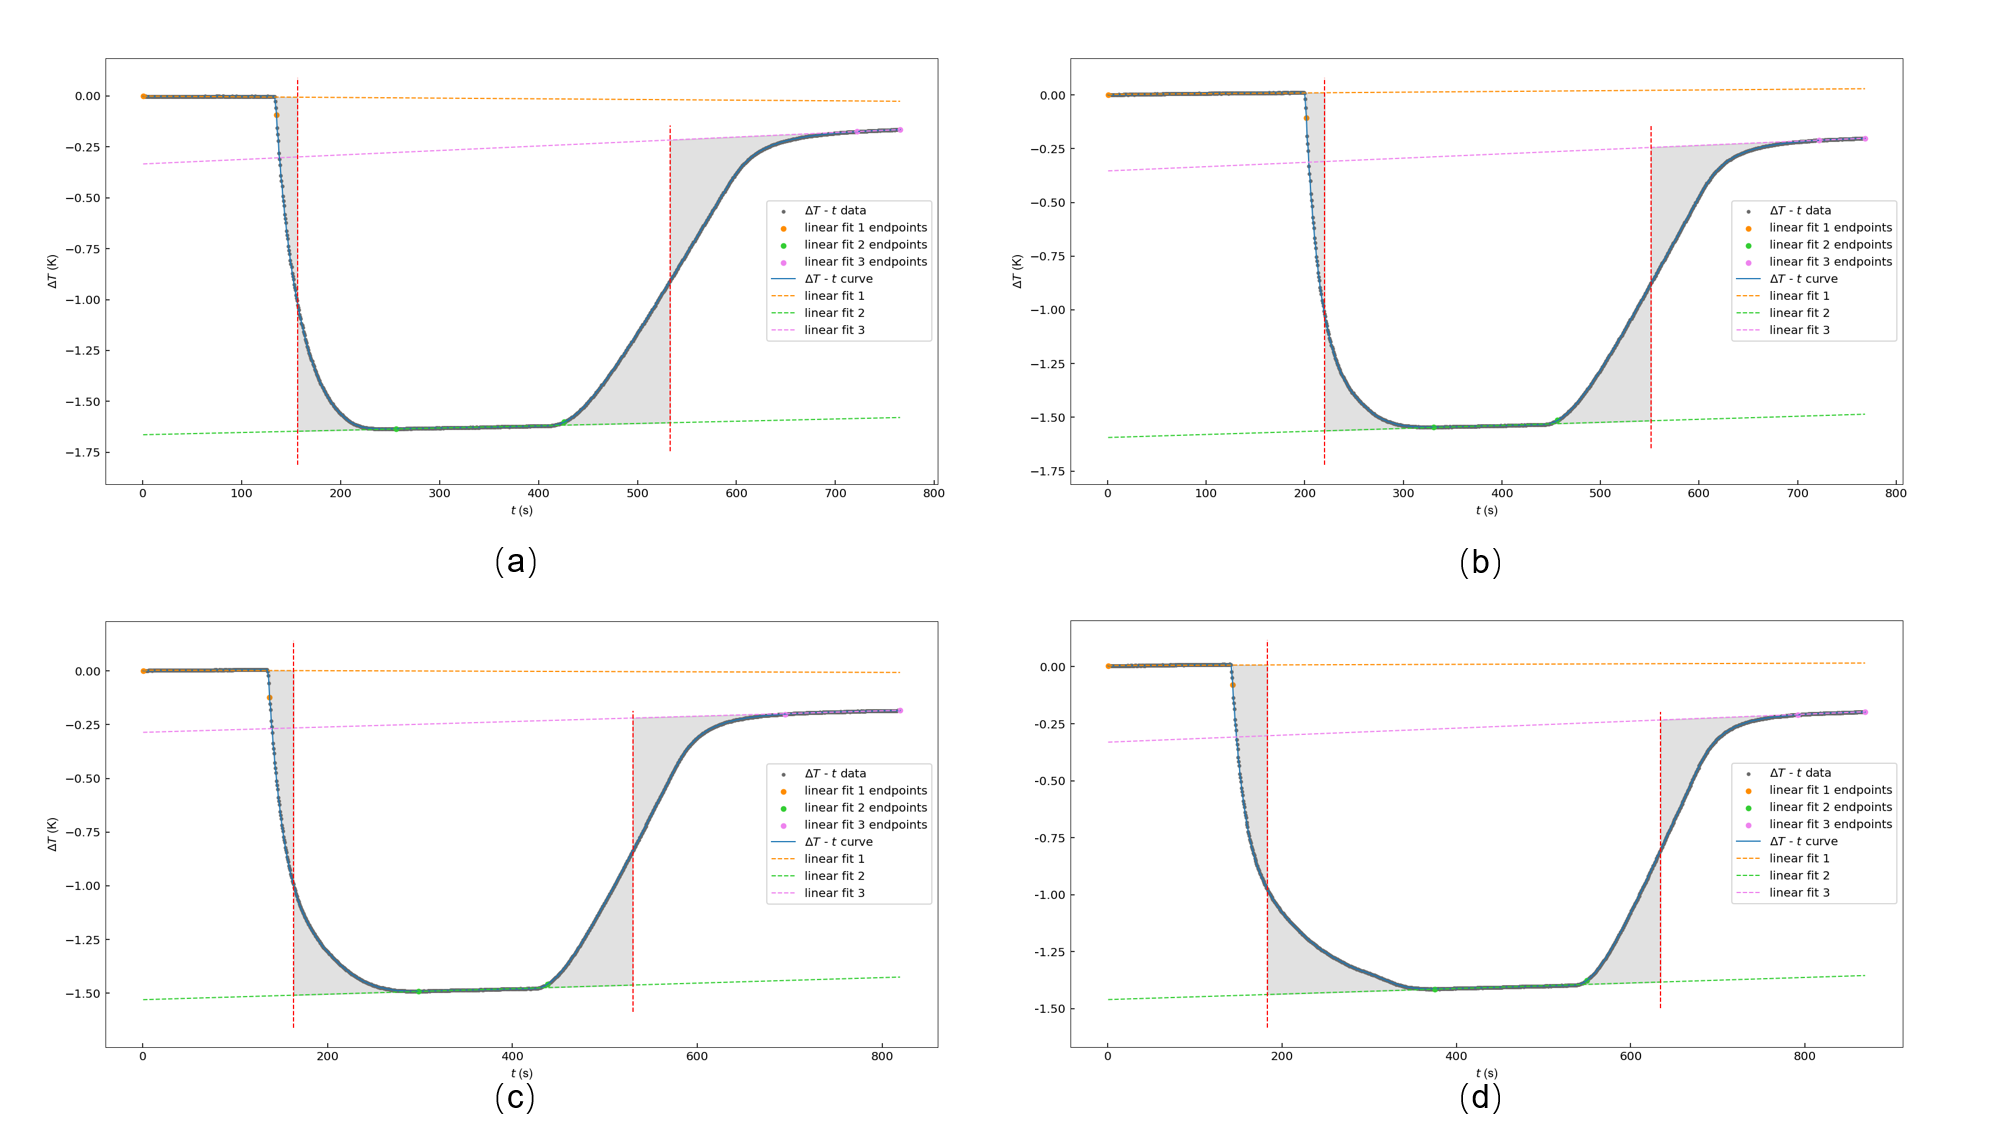
\includegraphics[width = \textwidth]{image/r1.png}
    \caption{第一轮实验温差随时间变化图( (a) - (d) 分别为第 1 至第 4 次实验)}\label{2}
\end{figure}

由公式 \ref{001} 可以计算在第一轮实验中各组的溶液浓度,如表 \ref{01} 所示。

\begin{table}[h]
    \centering
    \caption{第一轮实验加料后溶液浓度}
    \label{01}
    \begin{tabular}{cccc}
    \hline
    组&加入溶质质量/g & 总溶质质量/g & $n_0$   \\ \hline
    1&10.0230  & 10.0230 & 279.604 \\
    2&10.0123  & 20.0353 & 139.877 \\
    3&10.0272  & 30.0625 & 93.2215 \\
    4&9.9925   & 40.0550 & 69.9656 \\ \hline
    \end{tabular}
\end{table}

在加热时记录加热前电阻与加热后电阻以及加热电流,由公式
\begin{equation}
    Q = Q^, \frac{T_2-T_1}{T_2^,-T_1^,}
\end{equation}
\begin{equation}
    Q^, = I^2Rt
\end{equation}
\begin{equation}
    Q_s = \frac{\sum Q}{\sum n_2}
\end{equation}

可以计算得到体系吸收的热量 $Q$ 和积分溶解热 $Q_s$,如表 \ref{02} 。

\begin{table}[h]
    \centering
    \caption{第一轮实验溶解热计算}
    \label{02}
    \begin{tabular}{cccccccc}
    \hline
    组&电流/A & $R_{before}$/$\rm \Omega$ & $R_{after}$/$\rm \Omega$ & 加热时间/s & $Q'$/kJ & $Q$/kJ & $Q_s$/$\rm kJ \cdot mol^{-1}$ \\ \hline
    1&1.45 & 9.54 & 9.54 & 189.947 & 3.81 & 4.50 & 45.4 \\
    2&1.44 & 9.74 & 9.64 & 157.775 & 3.17 & 3.92 & 42.5 \\
    3&1.44 & 9.66 & 9.63 & 154.328 & 3.09 & 3.75 & 40.9 \\
    4&1.45 & 9.64 & 9.64 & 139.233 & 2.82 & 3.55 & 39.7 \\ \hline
    \end{tabular}
\end{table}

作出$1/Q_s-1/n_0$图,如图 \ref{3} ,得到线性关系如下。
\begin{equation}\label{-1}
    Q_s^{-1} = (0.0212 \pm 0.0003) + (0.29 \pm 0.03) * n_0^{-1} \quad R^2=0.961
\end{equation}

\begin{figure}[htbp]
    \centering
    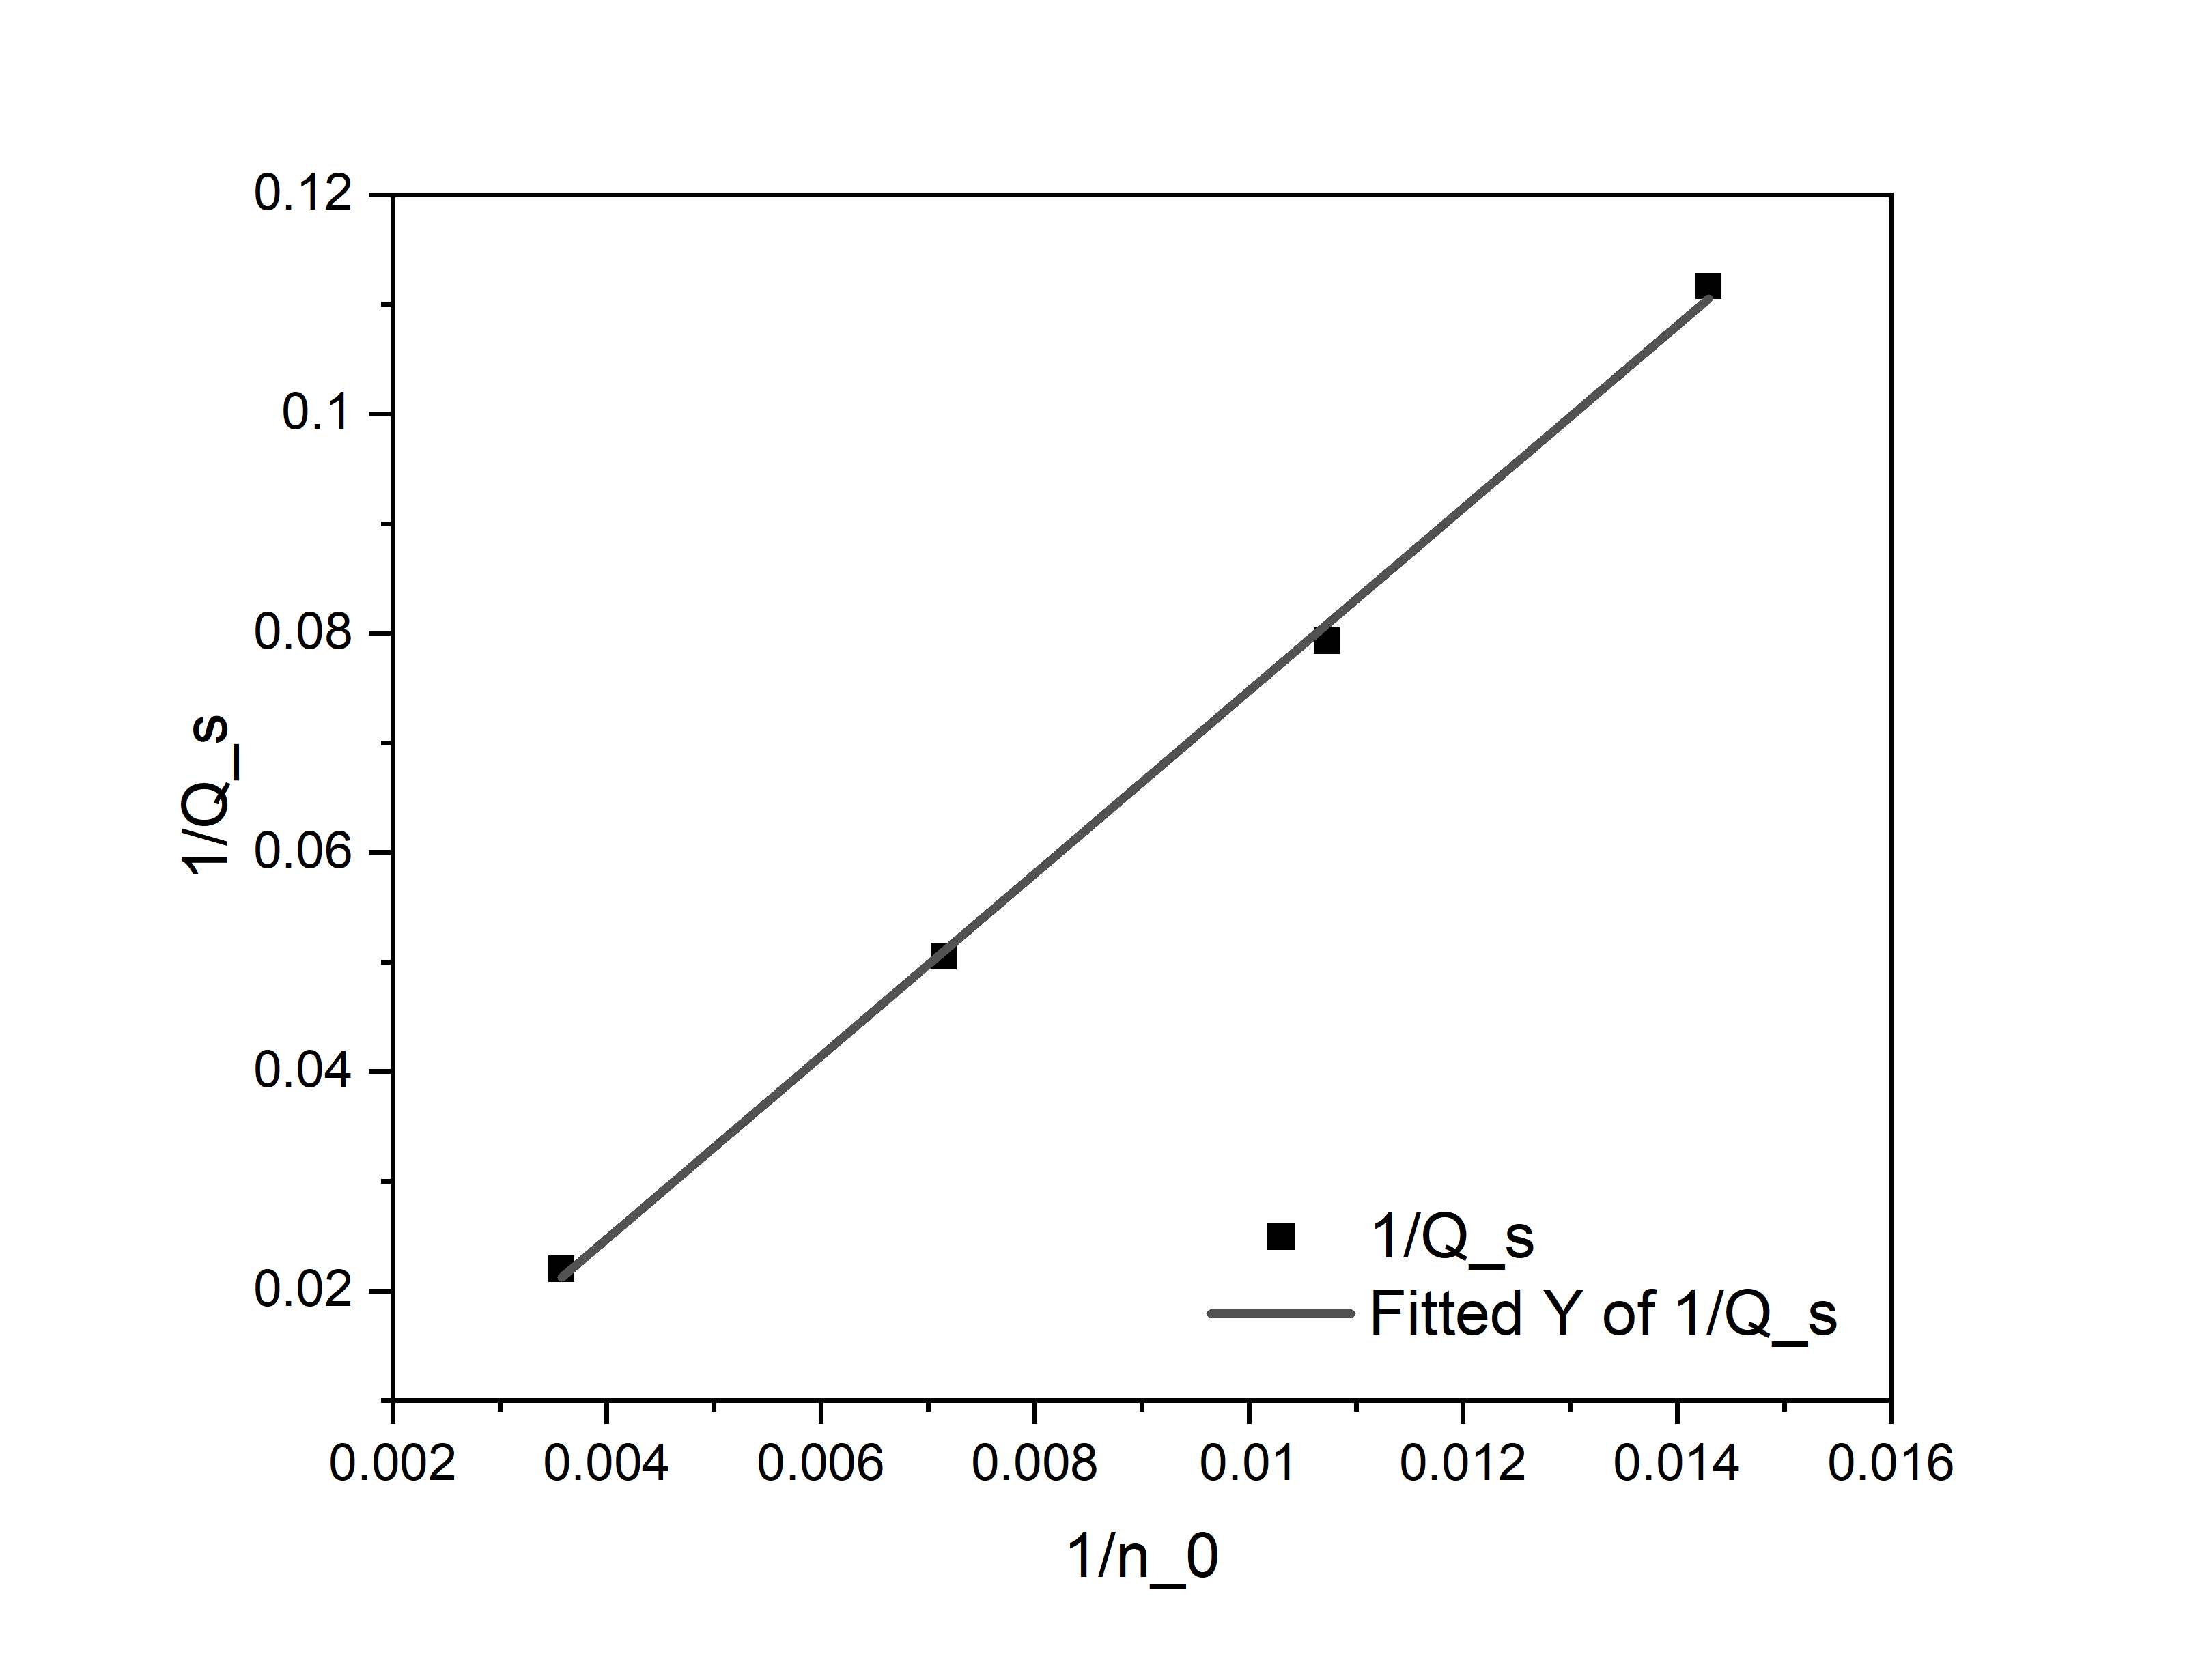
\includegraphics[width = 0.70\textwidth]{image/Graph4.png}
    \caption{第一轮实验$Q_s^{-1}-n_0^{-1}$图}\label{3}
\end{figure}
\subsection{第二轮实验}
为使加料次序让$n_0$的上升更为平稳,笔者先在去离子水中加入 10 g 硝酸钾,再
依次加入 3 g, 3 g, 4 g, 7 g, 13 g, 30 g 硝酸钾。记录温度-时间关系图如图 \ref{4} 。

\begin{figure}[htbp]
    \centering
    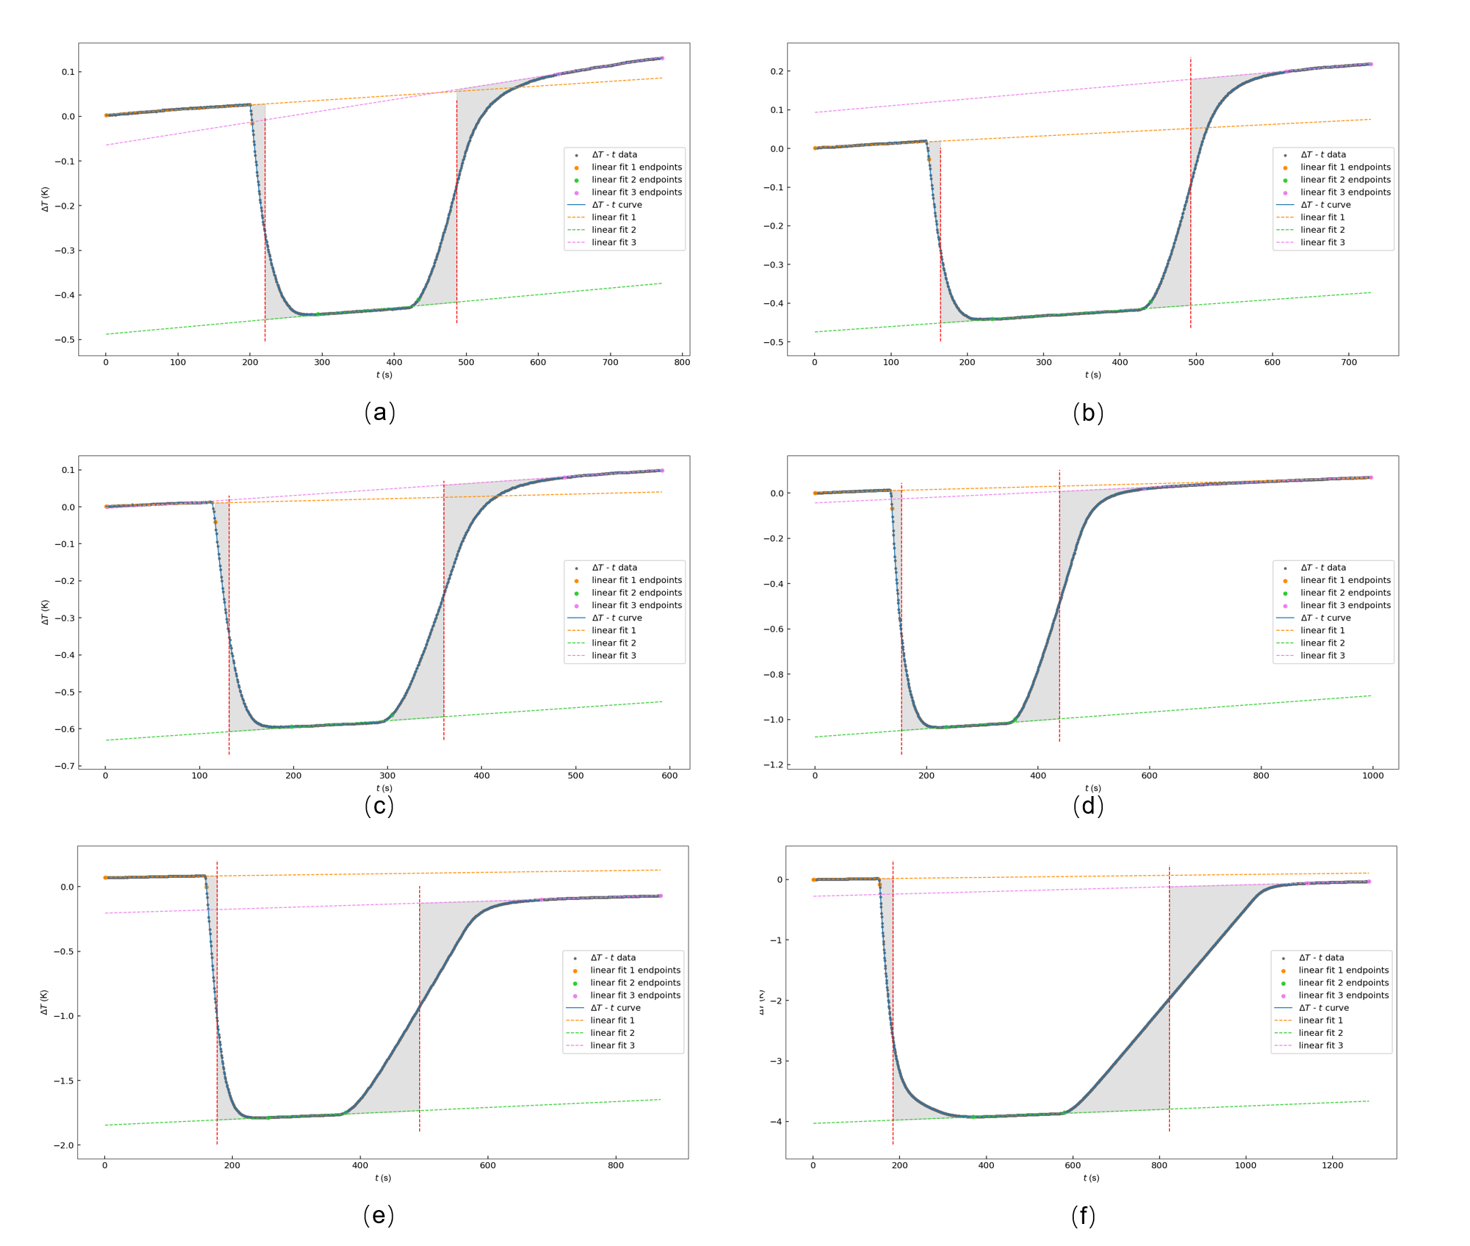
\includegraphics[width = \textwidth]{image/r2.png}
    \caption{第二轮实验温差随时间变化图( (a) - (f) 分别为第 1 至第 6 次实验)}\label{4}
\end{figure}

由公式 \ref{001} 可以计算在第二轮实验中各组的溶液浓度,如表 \ref{03} 所示。

\begin{table}[h]
    \centering
    \caption{第二轮实验加料后溶液浓度}
    \label{03}
    \begin{tabular}{cccc}
    \hline
    组&加入溶质质量/g & 总溶质质量/g & $n_0$    \\ \hline
    1&3.0175   & 13.0408 & 214.900  \\
    2&2.9935   & 16.0343 & 174.780  \\
    3&3.9934   & 20.0277 & 139.930 \\
    4&7.0105   & 27.0382 & 103.649 \\
    5&13.0288  & 40.0670  & 69.9450   \\
    6&29.9935  & 70.0605 & 40.0010   \\ \hline
    \end{tabular}
\end{table}

同样地,也可以计算得到体系吸收的热量 $Q$ 和积分溶解热 $Q_s$,如表 \ref{02} 所示。

\begin{table}[h]
    \centering
    \caption{第二轮实验溶解热计算}
    \label{04}
    \begin{tabular}{cccccccc}
    \hline
    组&电流/A & $R_{before}$/$\rm \Omega$ & $R_{after}$/$\rm \Omega$& 加热时间/s & $Q'$/kJ & $Q$/kJ& $Q_s$/$\rm kJ \cdot mol^{-1}$ \\ \hline
    1&1.43 & 9.54 & 9.55 & 68.329  & 1.33 & 1.35& 45.4 \\
    2&1.43 & 9.52 & 9.50  & 77.207  & 1.50 & 1.21& 44.5 \\
    3&1.43 & 9.51 & 9.51 & 81.428  & 1.58 & 1.57& 43.5 \\
    4&1.43 & 9.51 & 9.52 & 125.516 & 2.44 & 2.58& 41.9 \\
    5&1.43 & 9.52 & 9.52 & 196.837 & 3.83 & 4.51& 39.6 \\
    6&1.43 & 9.51 & 9.50  & 446.152 & 8.67 & 9.43& 36.3 \\ \hline
    \end{tabular}
\end{table}

据此作出$1/Q_s-1/n_0$图,如图 \ref{5} ,得到线性关系如下。
\begin{equation}\label{-2}
Q_s^{-1} = (0.0210 \pm 0.0002) + (0.27 \pm 0.02) * n_0^{-1} \quad R^2=0.983
\end{equation}

\begin{figure}[htbp]
    \centering
    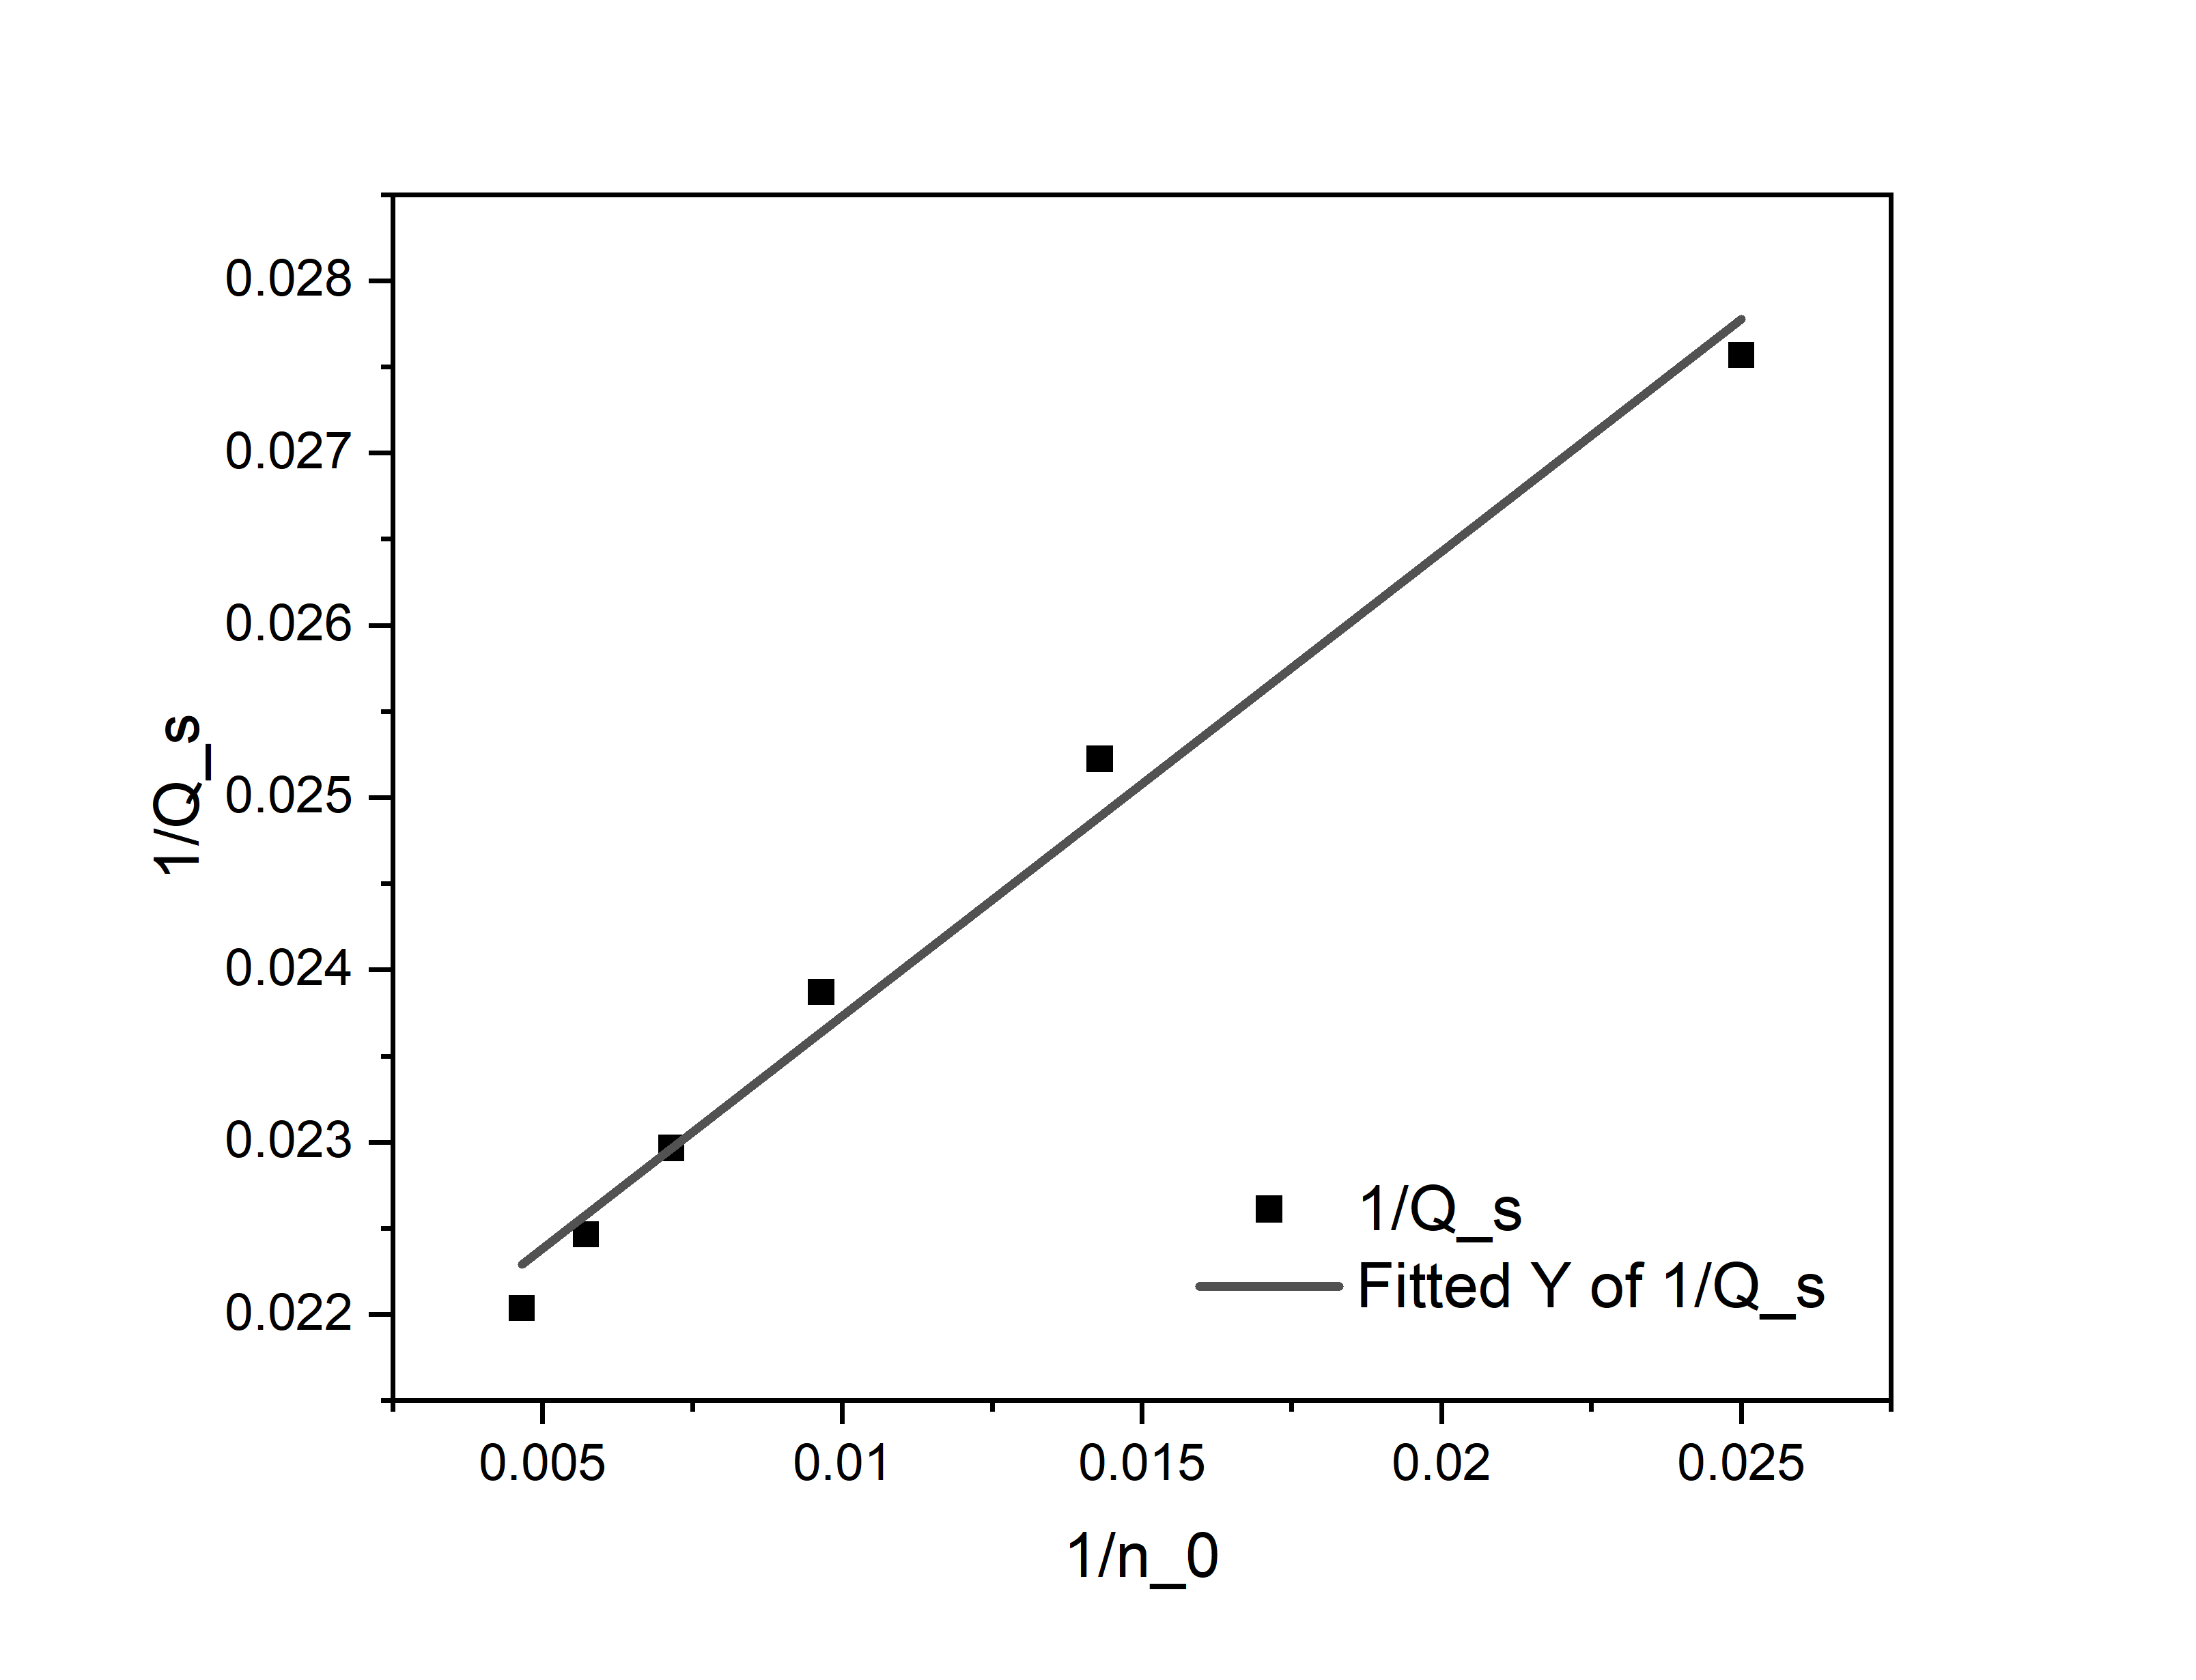
\includegraphics[width = 0.70\textwidth]{image/Graph7.png}
    \caption{第二轮实验$Q_s^{-1}-n_0^{-1}$图}\label{5}
\end{figure}

不使用课程提供的软件,笔者对第二组数据进行分段线性拟合,得到图像如图 \ref{6}
三段拟合直线方程如公式 \ref{002}  - \ref{004} ,方程的斜率分别为 $k_1, k_2, k_3$。
\begin{equation}\label{002}
    T = (0.00120 \pm 0.00006) + (1.263 \times 10^{-4} \pm 7 \times 10^{-7}) * t \quad R^2=0.993
\end{equation}
\begin{equation}\label{003}
    T = (-0.4697 \pm 0.0002) + (1.248 \times 10^{-4} \pm 5 \times 10^{-7}) * t \quad R^2=0.996
\end{equation}
\begin{equation}\label{004}
    T = (-0.082 \pm 0.002) + (1.89 \times 10^{-4} \pm 2 \times 10^{-6}) * t \quad R^2=0.975
\end{equation}
\begin{figure}[htbp]
    \centering
    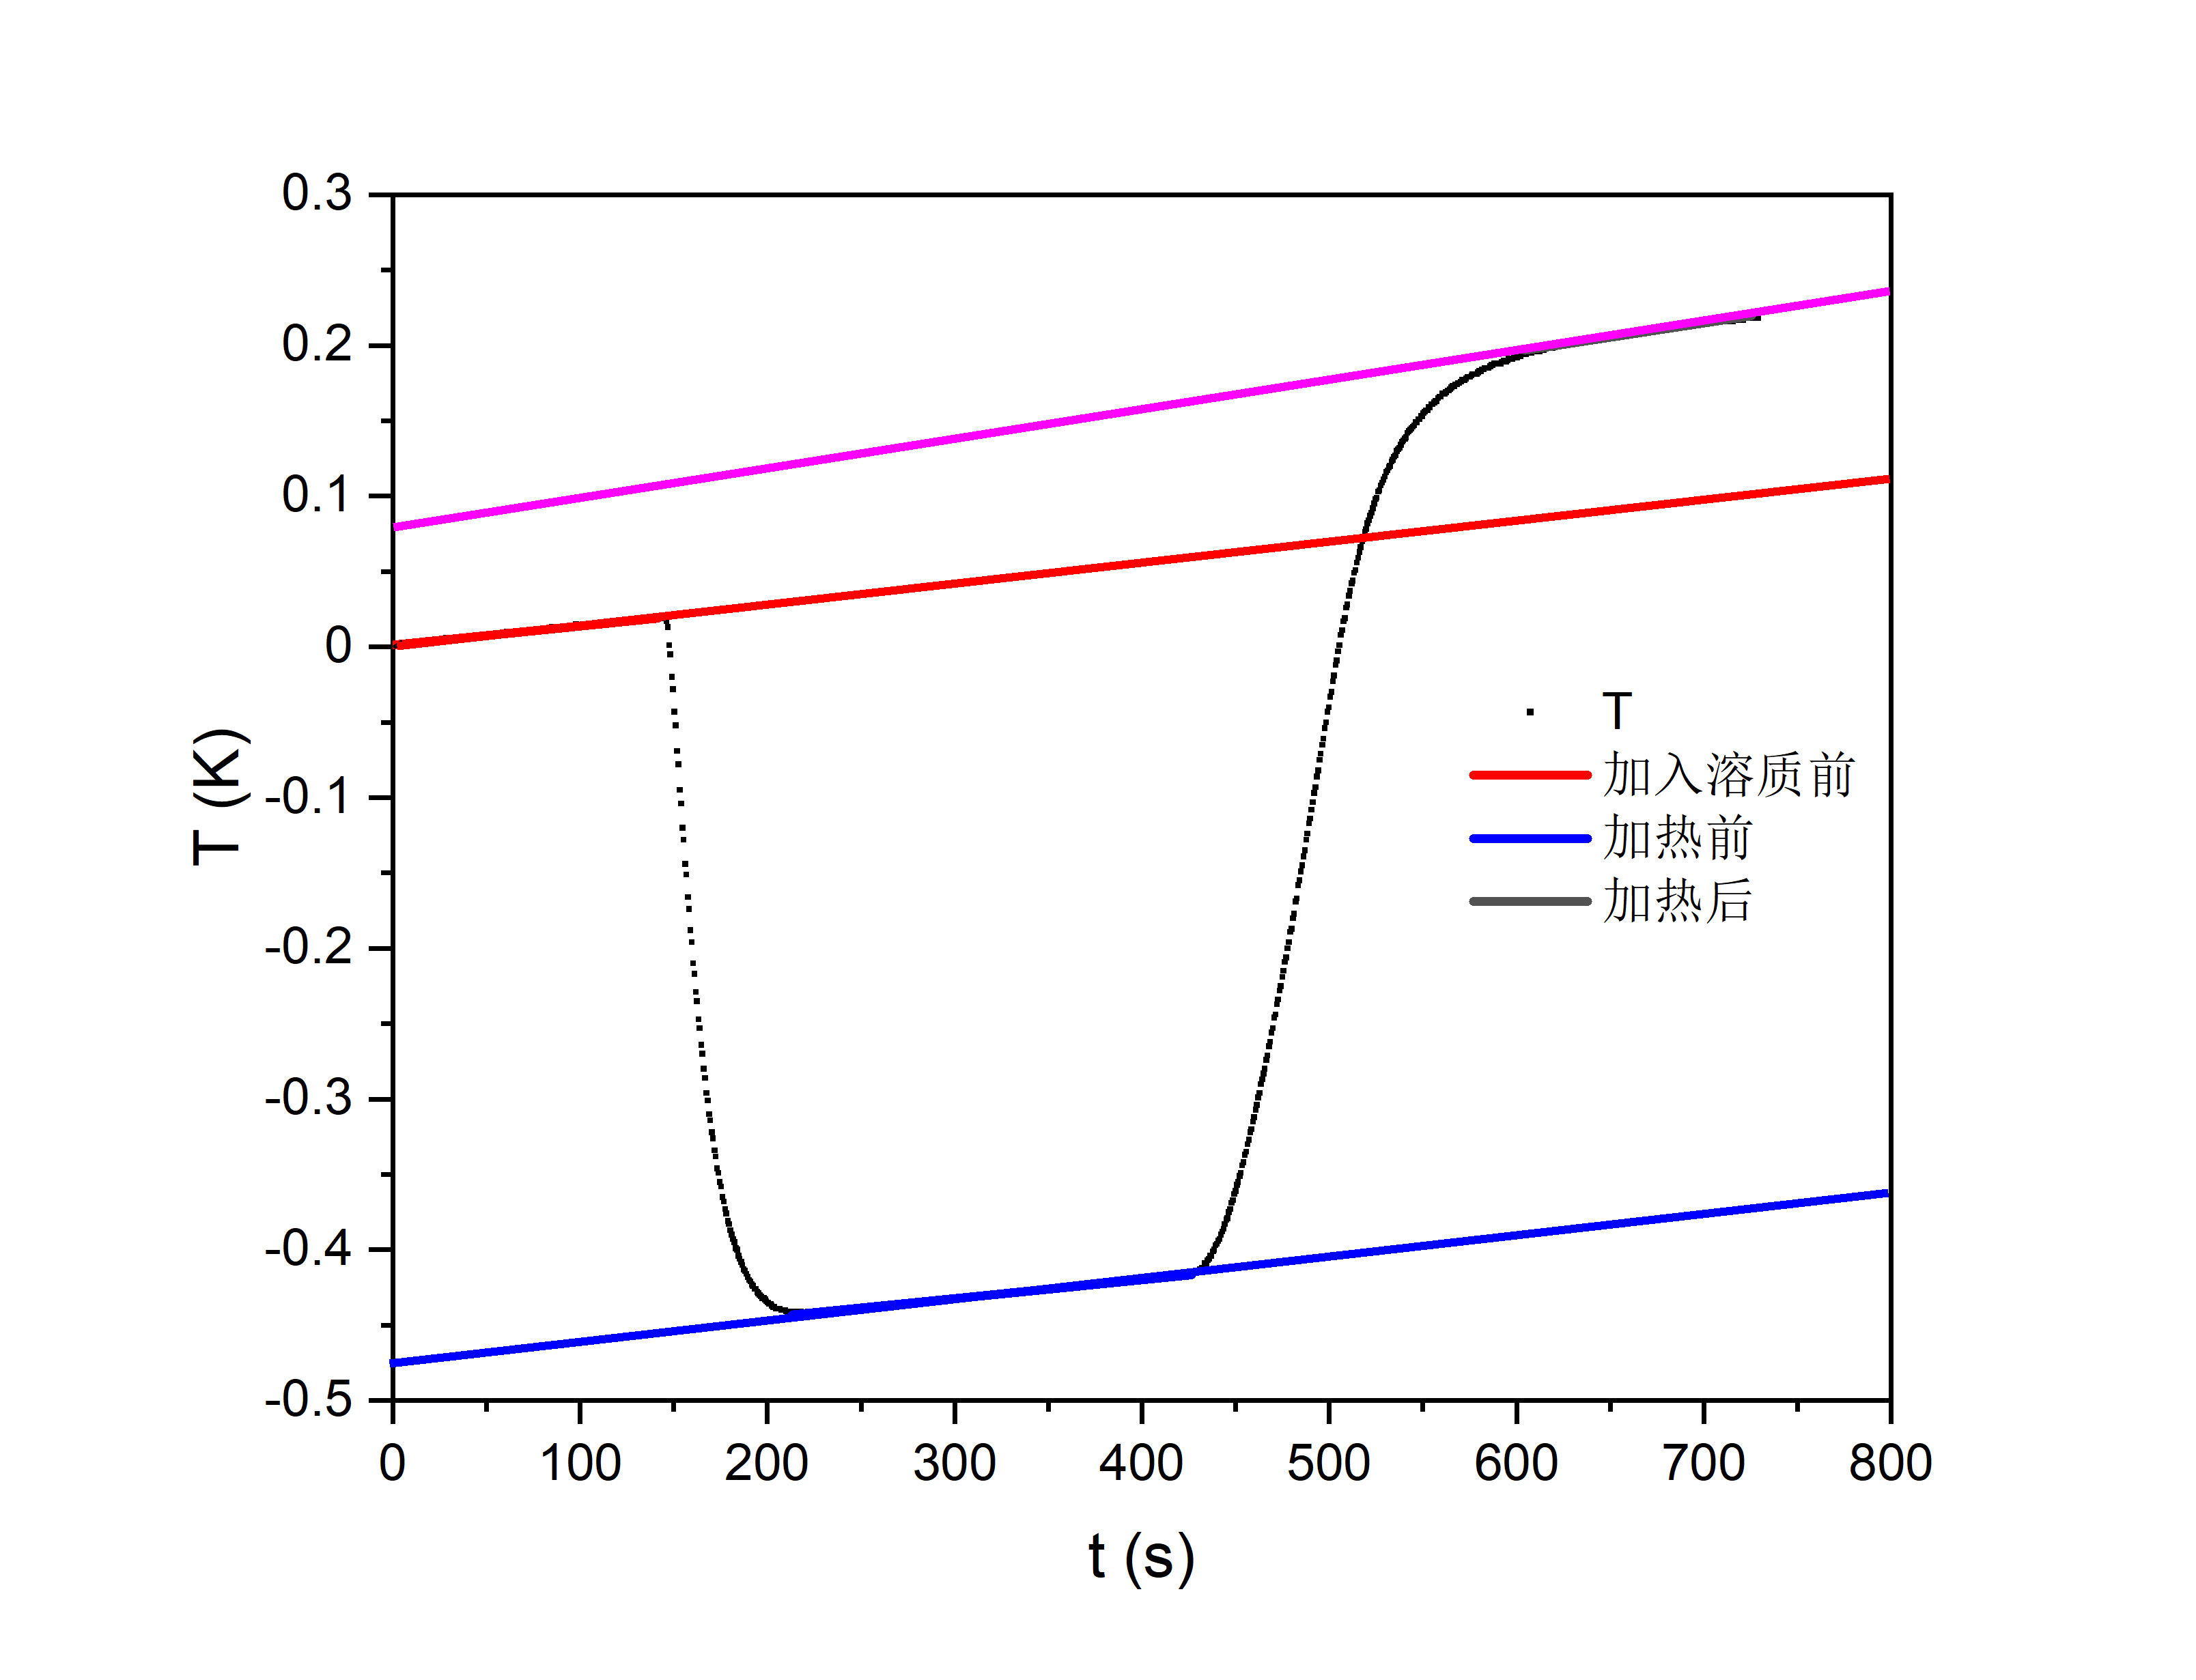
\includegraphics[width = 0.70\textwidth]{image/Graph8.png}
    \caption{第二轮实验第 2 次温差随时间变化图}\label{6}
\end{figure}
对于加料引起的降温过程,环境引起的升温速率可以使用 $k_1$ 和 $k_2$ 的平均值 $\bar{k_{a}}$ 
表示。而对于电加热过程中环境引起的升温速率,环境引起的升温速率可以使用 $k_3$ 和 $k_2$ 的平均值 $\bar{k_{b}}$
表示。平台期间的温度差可由公式 \ref{007} 得到。
\begin{equation}\label{005}
    \bar{k_{a}} = \frac{k_1 + k_2}{2} = \frac{1.263 \times 10^{-4} + 1.248 \times 10^{-4}}{2} = 1.256 \times 10^{-4}\ K/s
\end{equation}
\begin{equation}\label{006}
    \bar{k_{b}} = \frac{k_2 + k_3}{2} = \frac{1.89 \times 10^{-4} + 1.248 \times 10^{-4}}{2} = 1.569 \times 10^{-4}\ K/s
\end{equation}
\begin{equation}\label{007}
    \Delta T_{ij} = |(T_j-T_i) - \bar{k_{ij}} \cdot (t_j - t_i)|
\end{equation}

\begin{table}[]
    \centering
    \caption{第二轮实验温差计算}
    \label{06}
    \begin{tabular}{cccc}
    \hline
    t/s     & $T$/K  & $\bar{k_ij}$/$K \cdot s^{-1}$         & $\Delta T_{ij}$/K                  \\ \hline
    143.337 & 0.019  & \multirow{2}{*}{1.26$\times 10^{-4}$} & \multirow{2}{*}{0.472} \\
    244.390 & -0.440 &                                       &                               \\
    393.033 & -0.421 & \multirow{2}{*}{1.57$\times 10^{-4}$} & \multirow{2}{*}{0.586}  \\
    639.219 & 0.204  &                                       &                               \\ \hline
    \end{tabular}
\end{table}

由于第二组 $Q^, = 1.50 kJ$ ,通过温差可以计算得到
$$
    Q = Q^, \frac{\Delta T_{12}}{\Delta T_{23}} = 1.21\ kJ
$$

在课程提供软件中使用了雷诺校正得到温度差,而笔者拟合时未使用雷诺校正,
得到结果与通过软件计算相同。因此可以说明在溶解热实验中与环境的热交换影响不大。

\section{实验结果与讨论}
\subsection[short]{讨论}
\subsubsection[short]{第一轮实验}

在第一轮实验中,每次加入的溶质的量相同。计算溶解降温的温差与电热丝升温的温差如表 \ref{07} 所示。可以看出
溶解降温的温差每组并不相同,且呈现递降的趋势。

\begin{table}[h]
    \centering
    \caption{第一轮实验温差计算}
    \label{07}
    \begin{tabular}{cccccc}
    \hline
    $T_1$/K & $T_2$/K & $T_3$/K & $T_4$/K & $\Delta T_1$/K & $\Delta T_2$/K \\ \hline
    -0.006  & -1.647  & -1.605  & -0.216  & 1.641          & 1.389          \\
    0.01    & -1.563  & -1.516  & -0.244  & 1.573          & 1.272          \\
    0.001   & -1.509  & -1.462  & -0.219  & 1.510           & 1.243          \\
    0.008   & -1.438  & -1.383  & -0.233  & 1.446          & 1.150           \\ \hline
    \end{tabular}
\end{table}

为得到较好的数据,我们采用梯度加料的方法,保证每一段的 $n_0$ 变化相同。加料顺序详见实验步骤。
率先加入的 10 g 硝酸钾所造成的的热效应使用了第一轮的数据计算。
\subsubsection[short]{第二轮实验}

实验结束后,可以绘制第二轮的$Q_s-n_0^{-1}$图,拟合得到图像如图\ref{8},得到拟合曲线如下
\begin{equation}
    Q_s = (46.7 \pm 0.5) + (4.4 \times 10^2 \pm 4 \times 10^1) * n_0^{-1} \quad R^2=0.960
\end{equation}

可以看出线性程度不佳,若剔除第六组数据得到
\begin{equation}
    Q_s = (47.8 \pm 0.3) + (5.9 \times 10^2 \pm 3 \times 10^1) * n_0^{-1} \quad R^2=0.987
\end{equation}

绘制其 95\% 置信区间,可以看出第六组数据不在前五组数据线性拟合的 95\% 置信区间内,因此应当剔除,最后一组数据偏离线性。
\begin{figure}[htbp]
    \centering
    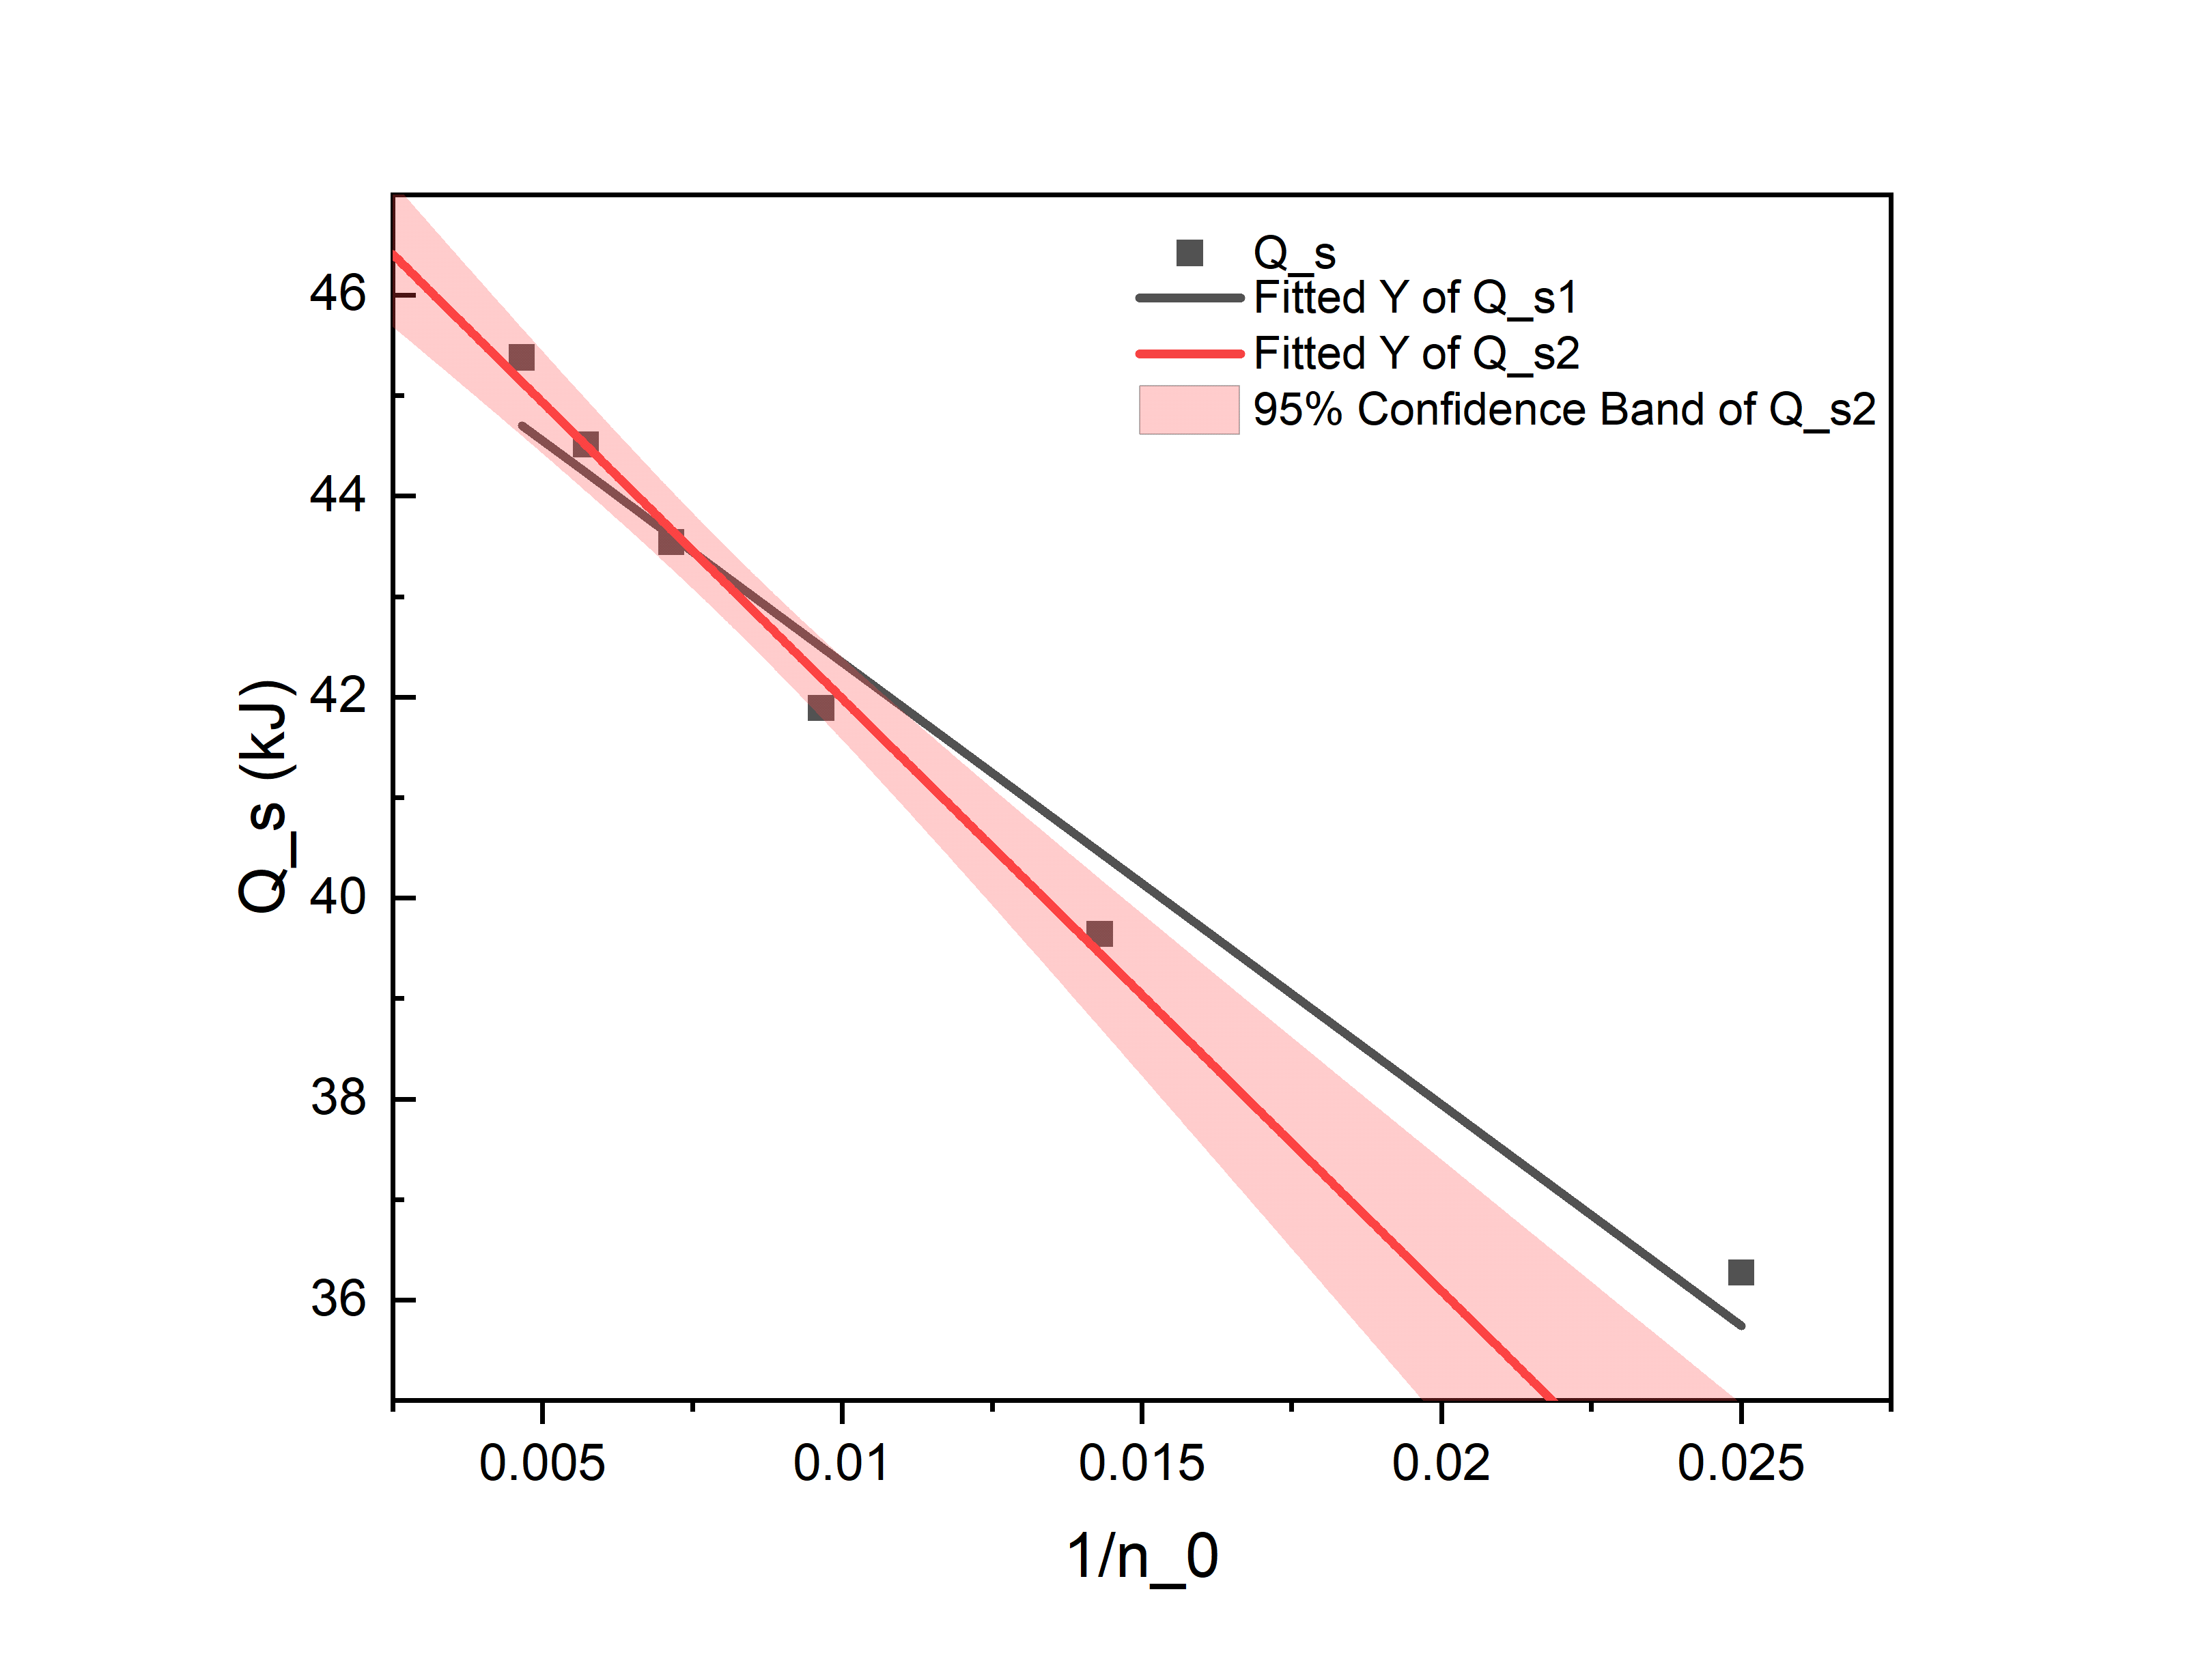
\includegraphics[width = 0.70\textwidth]{image/Graph12.png}
    \caption{第二轮实验$Q_s-n_0^{-1}$图}\label{8}
\end{figure}


可以绘制第一轮和第二轮的$Q_s^{-1}-n_0^{-1}$图,如图 \ref{3} 和图 \ref{5},
线性拟合关系如公式 \ref{-1} 和 \ref{-2},且线性关系较好。由图像可以看出 $Q_s$ 随浓度上升而下降
其对应的微观机制为: 硝酸钾浓度越高,离子强度高,水的化学势降低,导致水和能的下降,因此 $Q_s$ 随浓度上升而下降
。

根据给出的 $Q_s$ 和 $n_0$ 的经验公式有:
\begin{equation}
    Q_s = Q_S^0 \frac{an_0}{1+an_0} \implies Q_s^{-1} = \frac{1}{Q_S^0 a} n_0^{-1} +\frac{1}{Q_S^0}
\end{equation}

对于第一轮实验可以计算得到
\begin{equation}
    Q_S^0 = \frac{1}{b} = 47.2 {\rm kJ/mol} \quad
    n_0 = \frac{b}{k} = 0.073 {\rm mol/kJ}
\end{equation}

对于第二轮实验可以计算得到
\begin{equation}
    Q_S^0 = \frac{1}{b} = 47.6 {\rm kJ/mol} \quad
    n_0 = \frac{b}{k} = 0.078 {\rm mol/kJ}
\end{equation}

可以绘制第一轮和第二轮的$Q_s-n_0$图,如图 \ref{9} ,拟合曲线可以参考公式 \ref{-2}。
由拟合曲线可以利用 GeoGebra 软件来绘制曲线,如图 \ref{10} 所示,可以计算微分冲淡热,微分溶解热和积分冲淡热
如下表 \ref{08} 所示。可以看出,微分溶解热逐渐趋近于 $Q_s$,微分冲淡热逐渐趋近于 0 。
\begin{figure}[htbp]
    \centering
    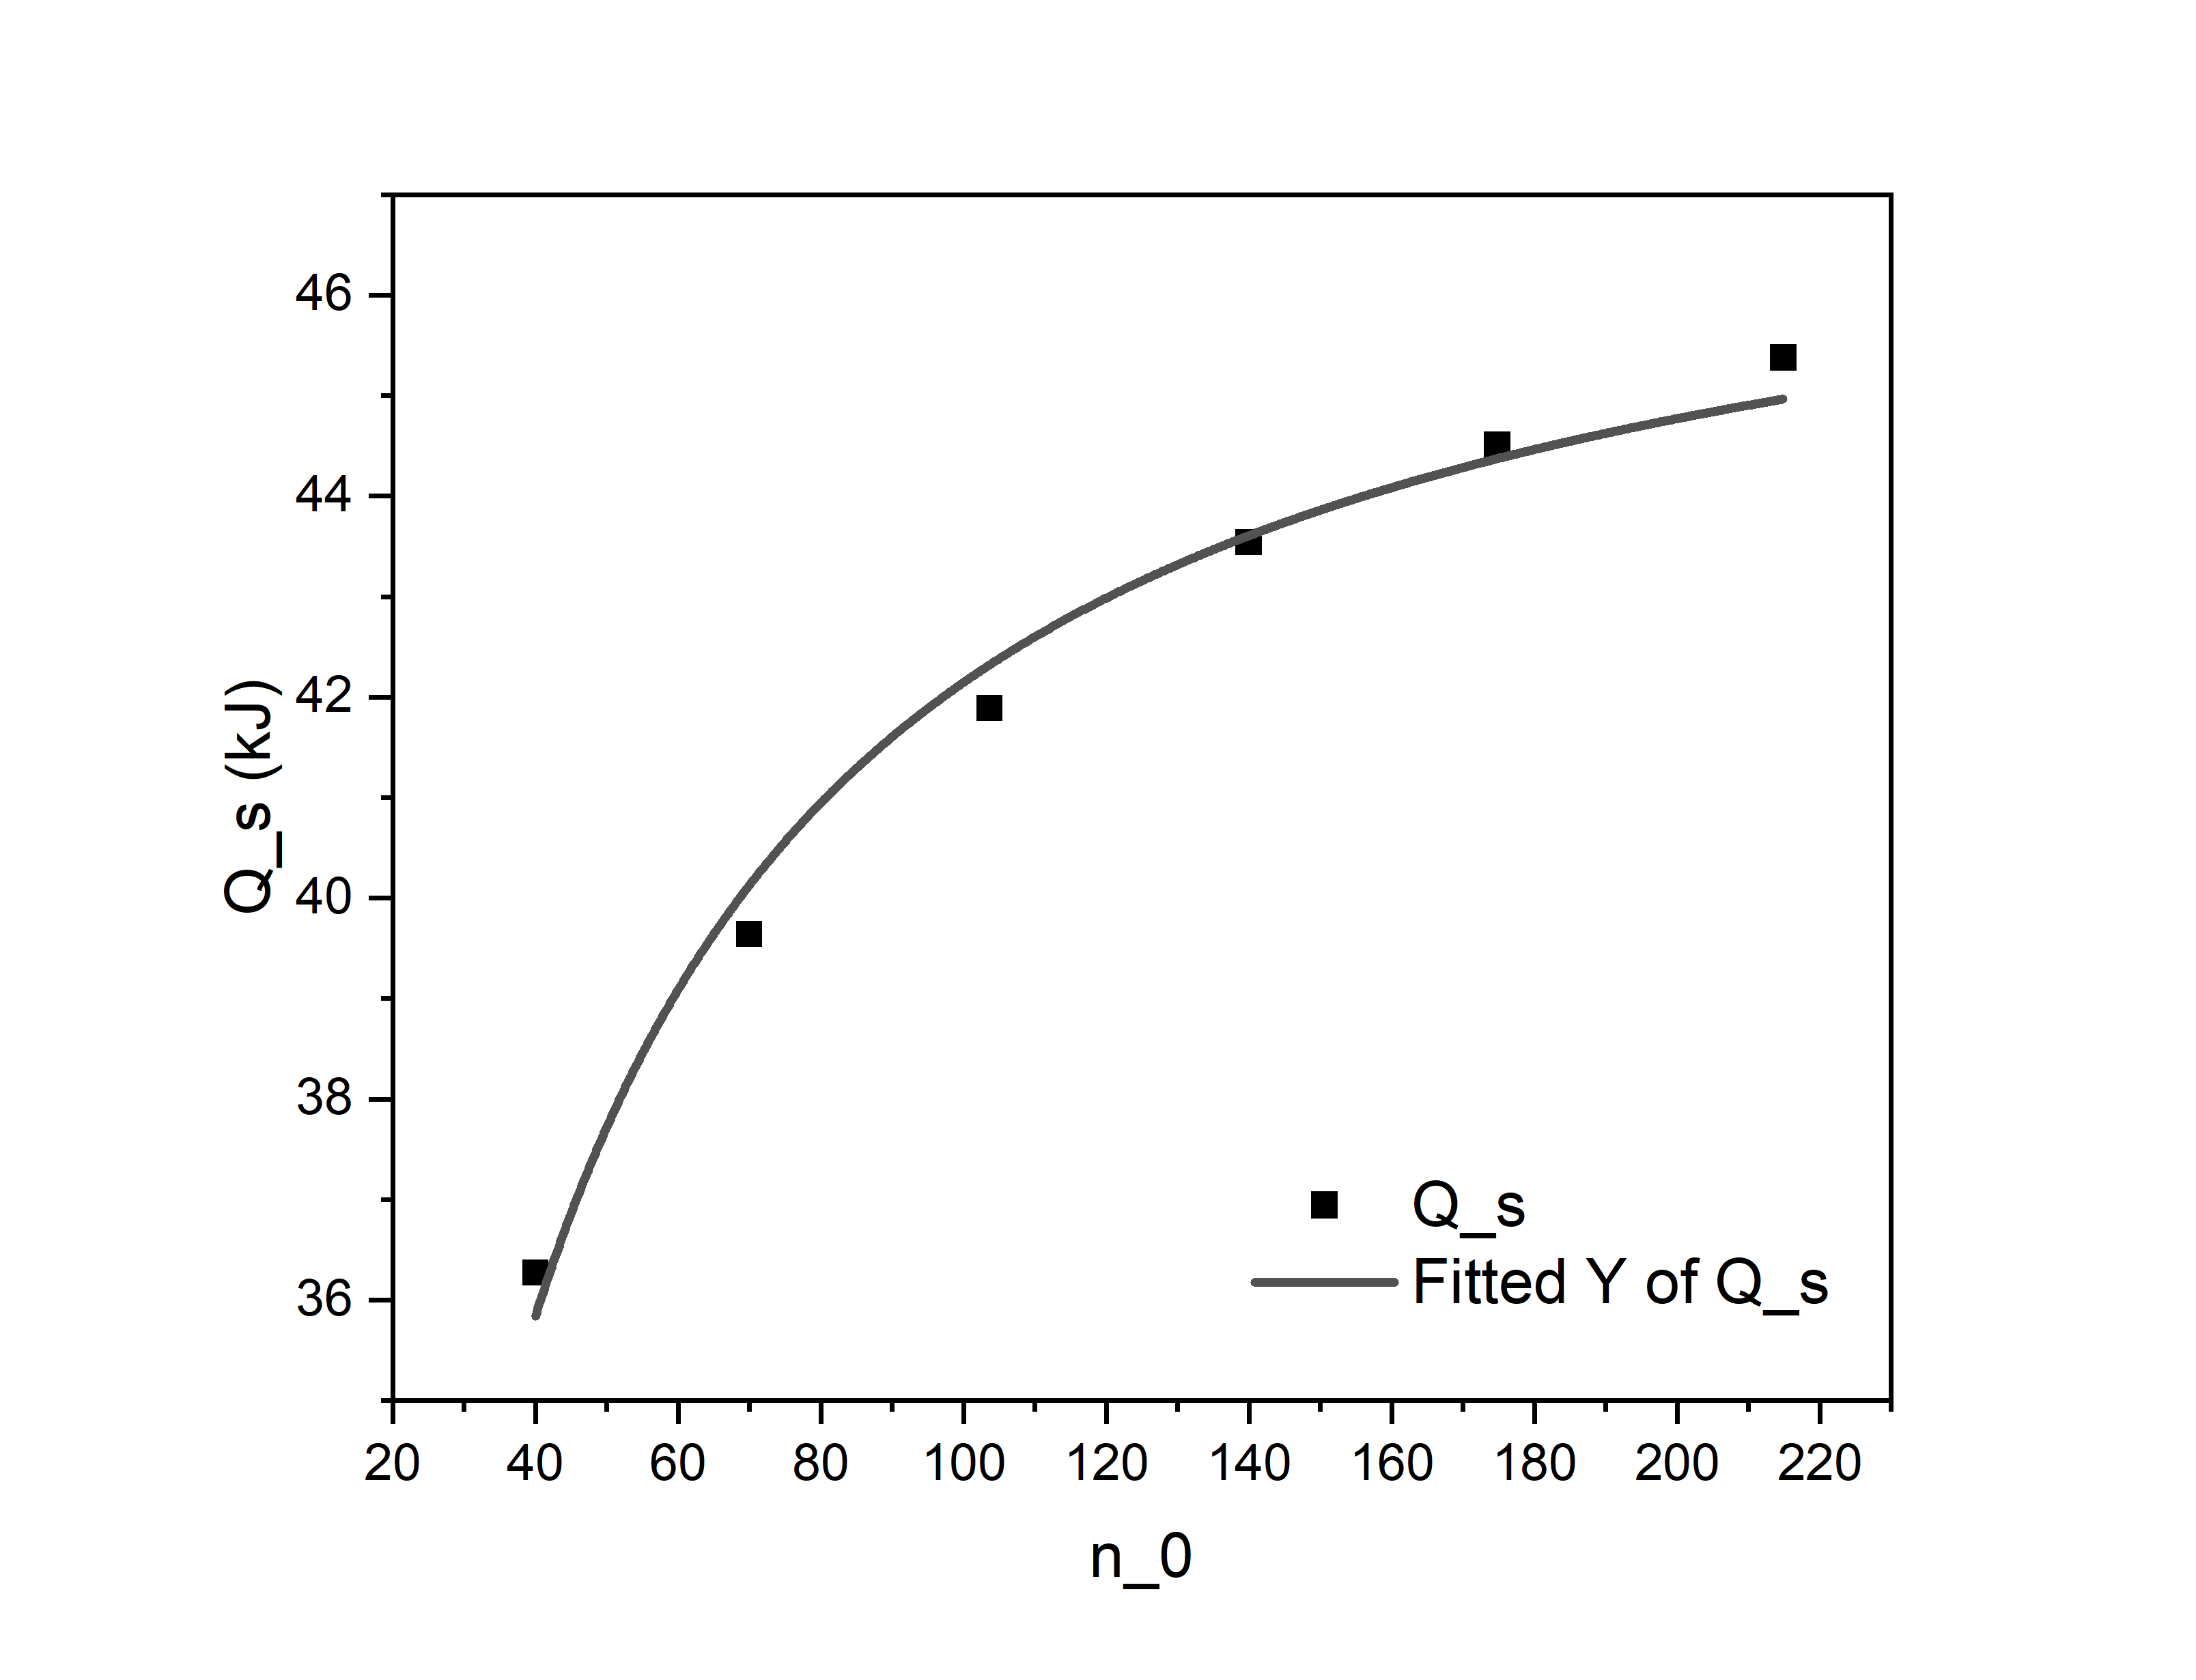
\includegraphics[width = 0.70\textwidth]{image/Graph13.png}
    \caption{第二轮实验$Q_s-n_0$图}\label{9}
\end{figure}

\begin{table}[h]
    \centering
    \caption{第二轮实验微分溶解热、微分冲淡热和积分冲淡热计算}
    \label{08}
    \begin{tabular}{cccc}
    \hline
    $n_0$ & 微分冲淡热/kJ & 微分溶解热/kJ & 积分冲淡热/kJ \\ \hline
    50    & 0.15     & 30.13    & 3.15     \\
    80    & 0.07     & 35.35    & 1.17     \\
    100   & 0.05     & 37.39    & 1.67     \\
    150   & 0.02     & 40.40    & 0.88     \\
    200   & 0.01     & 42.04    & --       \\ \hline
    \end{tabular}
\end{table}

\begin{figure}[htbp]
    \centering
    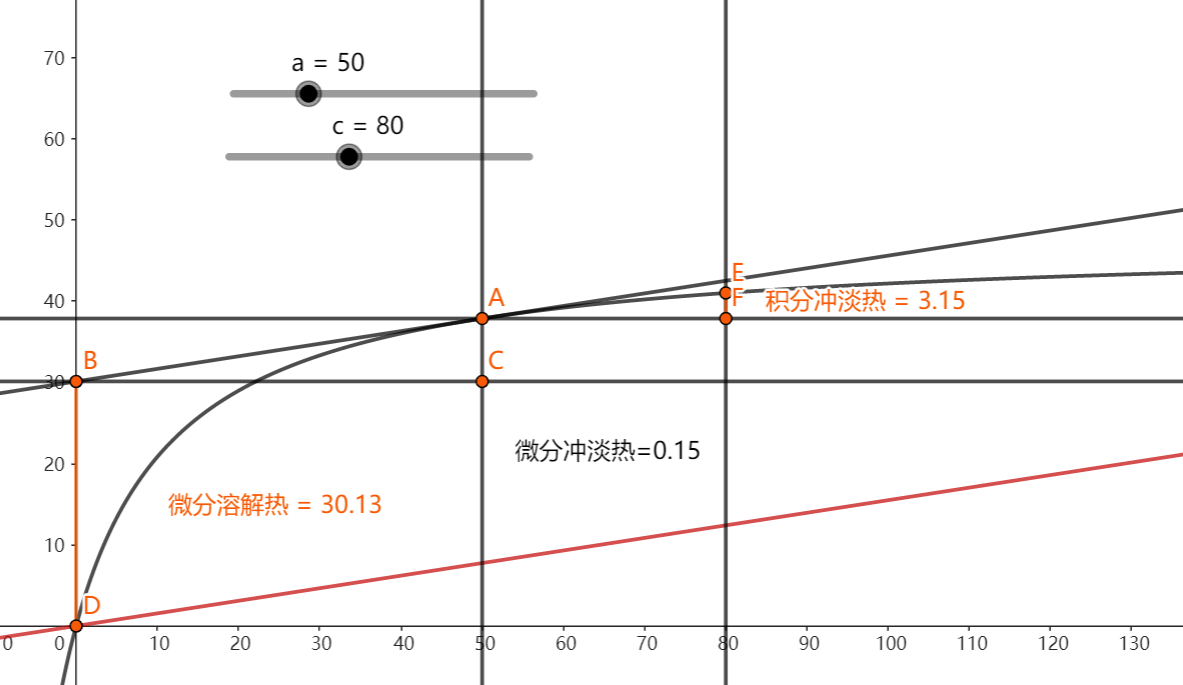
\includegraphics[width = 0.70\textwidth]{image/ggb.png}
    \caption{GeoGebra软件对微分溶解热、微分冲淡热和积分冲淡热计算($n_0^,=50, n_0^{,,}=80$)}\label{10}
\end{figure}

\subsubsection{与标准值的比较与误差分析}

由文献\cite{dk}可以得到硝酸钾无限稀溶液的溶解热为 37.25 $\rm kJ/mol$。
根据第二次实验可以得到无限稀溶液的溶解热为 47.2 $\rm kJ/mol$。
$$
E_r = \frac{37.25 - 42.7}{37.25} =  - 14.6 {\rm kJ/mol}
$$

可以看出误差较大,可能的误差来源有,电学量的测量的误差、各种物质的称量误差、温度和时间的读数误差以及体系与环境的热交换以及磁子搅拌做功造成的误差。
由于电学量以及称量误差相对可控,温度和时间都是通过软件自动给出,因此笔者认为主要的误差来源是由于体系与环境的热交换造成的。
又由于前文已经给出的是雷诺校正后的相关结果,因此雷诺校正并不能有效地改善测量的误差。


\subsection{结论}
本实验中,利用电热补偿法测定了硝酸钾在不同浓度的水溶液中的溶解热,绘制了 $T-t$ 图、$Q_s-n_0$ 图、$Q_s^{-1}-n_0^{-1}$ 图以及 $Q_s-n_0^{-1}$ 图,并拟合了 $Q_s^{-1}-n_0^{-1}$ 以及 $Q_s-n_0^{-1}$ 的线性关系。通过经验式,
得到 $Q_S^0 = 47.6 {\rm kJ/mol} $、$
n_0  = 0.078 {\rm mol/kJ}$
, 并与真实值相比较,并进一步地计算了其他溶解过程的热效应。

\nocite{*}
\bibliography{reference}
\end{document}
